%! Author = Philipp Emmenegger
%! Date = 30/06/2021

\section{Introduction}

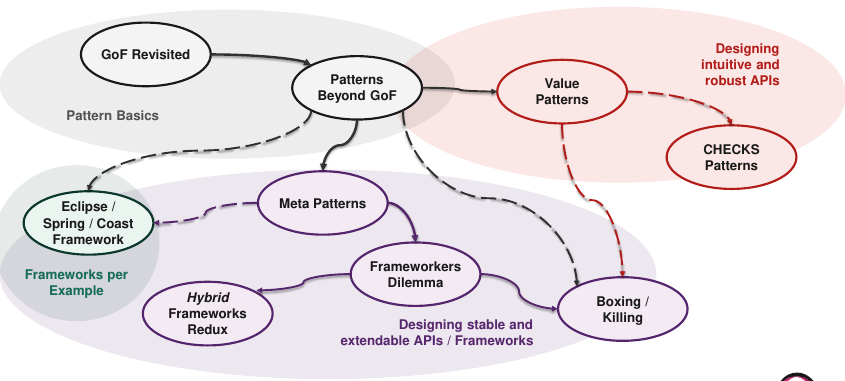
\includegraphics[width=\linewidth]{overview.png}

\subsection{Pattern Definition}
Beschreibung von erfolgreichen Engineering Stories für eine allgemein bekannte Absicht (\textcolor{blue}{Intent})

\begin{itemize}
    \item Adressiert wiederkehrendes \textcolor{blue}{Problem}
    \item Beschreibt generische \textcolor{blue}{Solutions}
    \item Weist \textcolor{blue}{Forces} hin (Was macht das Problem schwer?)
    \item Legt die Konsequenzen bzw. \textcolor{blue}{Benefits} und \textcolor{blue}{Liabilities} (Verbindlichkeiten) offen
    \item haben \textcolor{blue}{Namen}
    \item \textcolor{blue}{Implementation} (Wie das Problem gelöst wird)
\end{itemize}

\subsection{Type of Patterns}
\begin{itemize}
    \item Architecture Patterns (Waiting Room)
    \item Software Patterns
    \begin{itemize}
        \item Design Pattern (Elements of Reusable Object-Oriented Sofware)
        \item Pattern-oriented Software Architecture (POSA)
    \end{itemize}
    \item Organizational Patterns
    \item Learning and Teaching Patterns
    \item Documentation Patterns
\end{itemize}

\subsection{What are Patterns not?}
\begin{itemize}
    \item Silver bullet
    \item Novices Tool
    \item Ready Made Components
    \item Means to turn off your brain
\end{itemize}
